\section{Background}
\label{sec:background}

\todo{write a short background about some of these concepts}

DSL?

Semi-qualitative modelling

Constraint programming

Factors, Criteria, Actions

Outcomes: help the stakeholders

\begin{itemize}
\item find alternative policies that can satisfy the goals,
\item identify inconsistencies in the problem definition,
\item  present visualisations of possible future trajectories.
\end{itemize}

The information from and for the stakeholders will go through at least
two layers of the GRACeFUL system before it reaches the constraint
solver. First, through the graphical visual interface, which will
assist the stakeholders in building the problem definition, and which
will present the results of the qualitative simulations, and second,
the DSLs which will translate between these interfaces and the
constraint programming layer.

GRACeFUL concept maps

TODO: use part of the commented text:

% The description of the system is elicited from stakeholders
% with help from the GRACeFUL system, which contains a library of relevant
% factors, relating them to the concepts under discussion. Here, the term
% \emph{factors} refers to \emph{characteristics of a system that can take
% a value, either quantitative or qualitative, that can change over time}
% (source: the \emph{GRACeFUL Glossary of Terms}). In mathematical system
% theory, a collection of factors correspond to the \emph{state} of the
% system. Similarly, \emph{external factors} correspond to \emph{inputs}
% to the system. As such, factors are assumed to be associated with
% measurable (if only in qualitative terms) values.
%
% As in systems theory, a distinction is made between inputs that are
% beyond the control of the system, and which are potentially uncertain
% (or even unknown), and \emph{actions} or combinations of actions, which
% represent the system theoretical \emph{controls}, generally assumed to
% be deterministic but with uncertain consequences.
%
% The interaction between the factors, and between the factors and the
% criteria, represents a first description of the system (no alternatives
% are present, or only the baseline policy is assumed to be active). This
% description is in the form of a \emph{causal loop diagram}. A causal
% loop diagram is a form of \emph{directed, simple, labelled graph}, i.e.:
%
% \begin{enumerate}
% \def\labelenumi{\alph{enumi}.}
% \item
%   a link between two nodes has a well-defined source and a target (it is
%   \emph{directed}); intuitively, the link represents a causal relation
%   between the source (cause) and the target (effect);
% \item
%   there can be at most one connection from one node to another (the
%   graph is \emph{simple}): either a causal relation exists, or it does
%   not. Note, however, that since the graph is directed, there may be an
%   inverse connection from the ``effect'' to the ``cause'', as in
%   feedback loops;
% \item
%   the connections are either \emph{positive} (an increase in the value
%   of the source causes an increase in the value of the target), or
%   \emph{negative} (an increase causes a decrease), hence the graph is
%   \emph{labelled}.
% \end{enumerate}
%
% It can be seen from the last point that nodes \emph{must} represent
% values that can be partially ordered. This rules out nodes that
% represent, say, stakeholders.
%
% As an example, two such causal loop diagrams, produced in the
% student sessions organised as part of the CRUD case study, can be
% found in the Appendix.
%
% The GRACeFUL system can assist in building the causal loop diagram, for
% example by suggesting connections, or by pointing out inconsistencies.
%
% At this stage, if we can attribute qualitative values to the various
% nodes, the causal loop diagram describes a system that can make the
% object of a qualitative simulation. The criteria play the roles of
% constraints: the qualitative trajectories that lead outside the criteria
% can be pruned by the constraint programming system.
%
% The causal loop diagram is enhanced to a GRACeFUL concept map by the
% addition of extra nodes and non-causal links. The extra nodes represent
% actions, goals, alternatives, and stakeholders.
%
% Like all previous elements, the actions are also obtained from the
% stakeholders. As explained in the previous section, actions are the
% components of alternatives, among which will be found the policy
% solutions we are seeking. Alternatives are, according to the GRACeFUL
% Glossary of Terms, ``action or combination of actions that influence the
% values of criteria''. They correspond to Walker's ``alternative
% policies'', where a \emph{policy} is defined ``loosely'' as ``a set of
% actions taken to solve a problem''. As in the case of goal definition,
% the GRACeFUL system can suggest such ``atomic actions'' that are useful
% to the goals in the context of the problem at hand.
%
% The role of actions in the GRACeFUL concept maps is to give initial
% values to the factors and criteria they influence. They do not link via
% causal loops to these factors, since actions are not of the requisite
% type (they do not represent values that can increase or decrease).
% However, they will usually have non-causal links, representing
% constraining relationships to the factors.
%
% In the other cases of extra nodes (goals, alternatives, and
% stakeholders), the links represent primarily ``belongs to''
% relationships: there are links from stakeholders to goals, indicating
% which stakeholders have declared which goals; there are links from goals
% to the criteria by which they are assessed; finally, there are links
% between alternatives and the factors and criteria that they (i.e., their
% constituent atomic actions) influence.
%
% Figure \ref{fig:cm} (drawn by Sadie McEvoy (Deltares)) shows a
% graphical representation of the structure of a GRACeFUL concept map:
%
% \begin{figure}[!ht]%
%   \centering
%  {{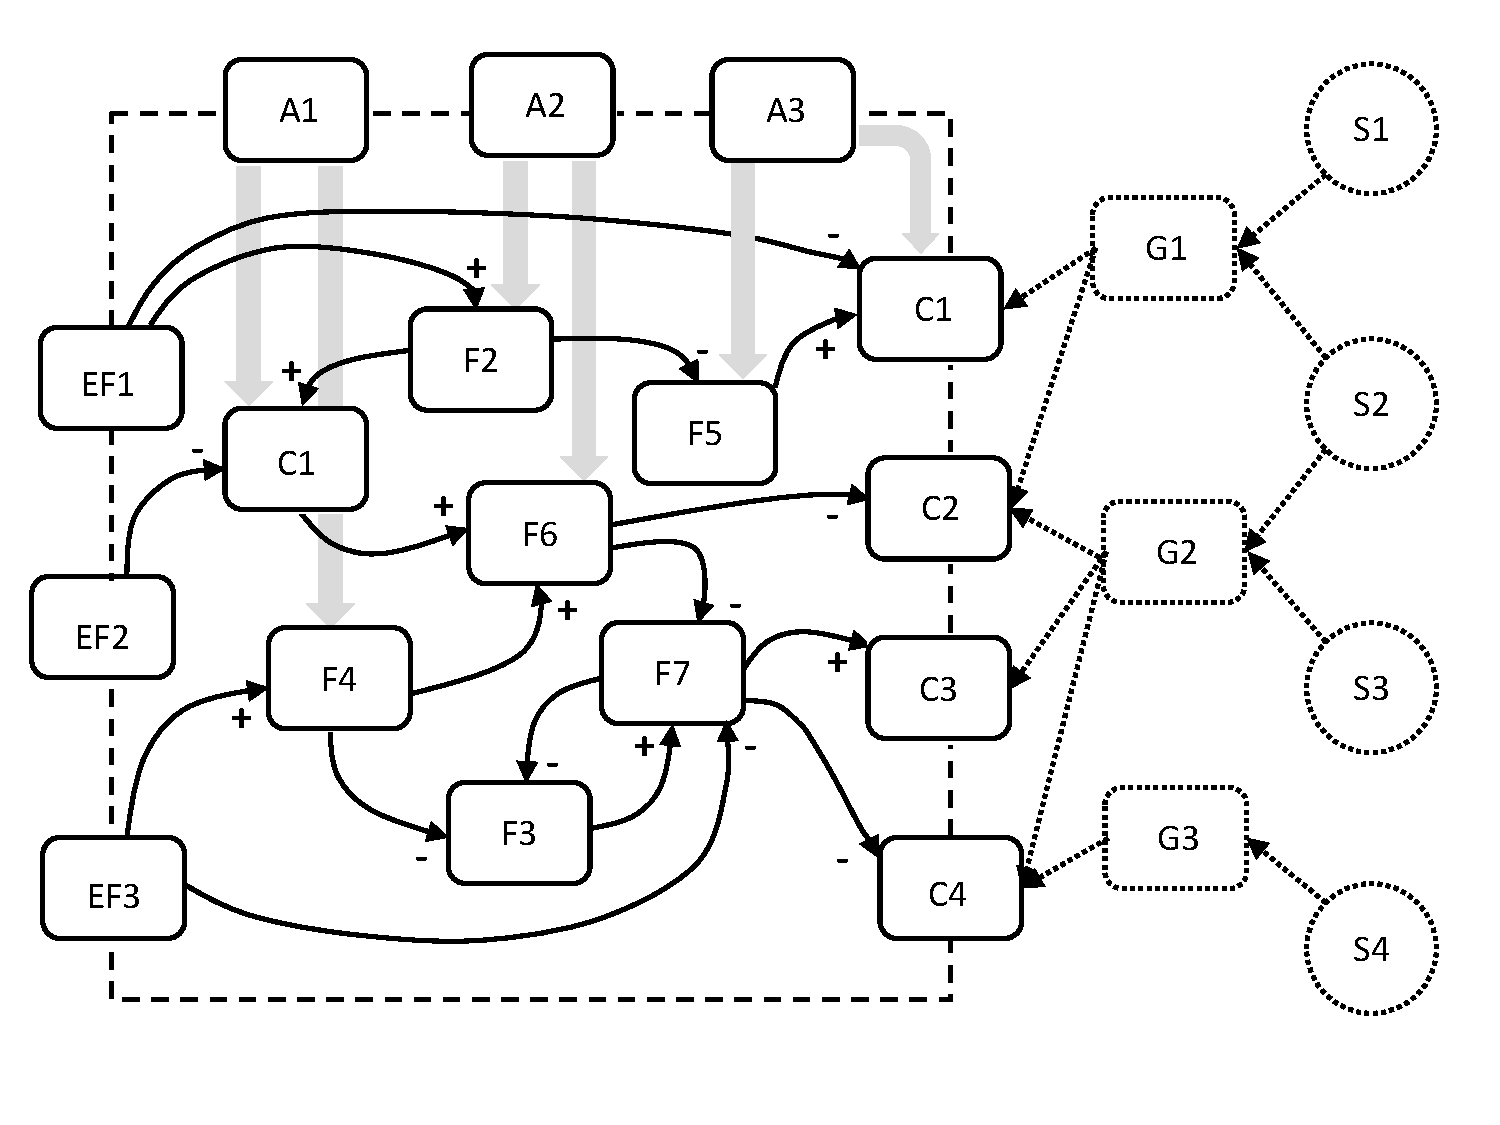
\includegraphics[width=0.9\textwidth]{../s4.pdf} }}%
%   \caption{The structure of a GRACeFUL concept map}%
%   \label{fig:cm}%
% \end{figure}

